\documentclass[10pt]{article}
\usepackage[polish]{babel}
\usepackage[utf8]{inputenc}
\usepackage[T1]{fontenc}
\usepackage{amsmath}
\usepackage{amsfonts}
\usepackage{amssymb}
\usepackage[version=4]{mhchem}
\usepackage{stmaryrd}
\usepackage{graphicx}
\usepackage[export]{adjustbox}
\graphicspath{ {./images/} }
\usepackage{hyperref}
\hypersetup{colorlinks=true, linkcolor=blue, filecolor=magenta, urlcolor=cyan,}
\urlstyle{same}

\title{PRACA KONTROLNA nr 3 - POZIOM PODSTAWOWY }

\author{}
\date{}


\begin{document}
\maketitle
\begin{enumerate}
  \item W trójkącie $A B C$ wpisanym w okrąg o środku $S$ i promieniu $r$ dany jest kąt $\alpha=\angle A B C$. Oblicz pole trójkąta $A S C$.
  \item Rozwią̇̇ równanie
\end{enumerate}

$$
|\sin x|+|\cos x|=\frac{\sqrt{6}}{2}
$$

\begin{enumerate}
  \setcounter{enumi}{2}
  \item Dana jest funkcja
\end{enumerate}

$$
f(x)=\cos \left(2 x-\frac{\pi}{6}\right)
$$

Narysuj starannie wykres funkcji $f(x)$. Rozwiąż nierówność $(f(x))^{2} \geqslant \frac{1}{2}$.\\
4. Niech $\alpha, \beta$ i $\gamma$ oznaczają kąty pewnego trójkąta. Wykaż, że jeżeli

$$
\frac{\sin \alpha}{\sin \beta}=2 \cos \gamma
$$

to ten trójkąt jest równoramienny.\\
5. Na okręgu o promieniu $r$ opisano trapez prostokątny, którego najkrótszy bok jest równy $\frac{4}{3} r$. Oblicz pole tego trapezu.\\
6. Pewną górę widać najpierw pod kątem $\alpha$ (jest to kąt między linią poziomą, a odcinkiem łączącym szczyt z obserwatorem), a po przybliżeniu się do niej o $d$ metrów widać ją pod nieco większym kątem $\beta$. Wyznaczyć względną wysokość tej góry. Wykonać obliczenia dla wartości $\alpha=41^{\circ}, \beta=45^{\circ}, d=90 \mathrm{~m}$.

\section*{PRACA KONTROLNA nr 3 - POZIOM RoZSZERZONY}
\begin{enumerate}
  \item Udowodnij, że
\end{enumerate}

$$
\cos 4 x=1-8 \cos ^{2} x+8 \cos ^{4} x
$$

Wykorzystując ten wzór, znajdź wartość $\cos \frac{\pi}{24}$.\\
2. Wykaż, że dla każdego trójkąta zachodzi nierówność

$$
\frac{1}{2 r}<\frac{1}{h_{a}}+\frac{1}{h_{b}}<\frac{1}{r},
$$

gdzie $h_{a}, h_{b}$ są wysokościami, a $r$ promieniem okręgu wpisanego w ten trójkąt.\\
3. Dana jest funkcja $f(x)=\sin 4 x \operatorname{ctg} 2 x-\frac{1}{2}$. Rozwiąż nierówność $f(x) \geqslant 1$ i narysuj staranny wykres $f(x)$.\\
4. Przekątne trapezu dzielą ten trapez na cztery trójkąty. Pola tych dwóch trójkątów, których bokami są podstawy trapezu równe są $S_{a}$ i $S_{b}$. Oblicz pole tego trapezu.\\
5. Manipulator robota składa się z dwóch ramion o długościach $l_{1} \mathrm{i} l_{2}$, połączonych przegubem. Pierwsze ramię umieszczono w początku układu współrzędnych.\\
Niech $\alpha$ oznacza kąt między pierwszym ramieniem i osią $O x$, a $\beta$ - kąt między drugim ramieniem i kierunkiem pierwszego ramienia (patrz rysunek). Wyznacz współrzędne końca drugiego ramienia (punktu $P$ ) w zależności od kątów $\alpha$ i $\beta$. Sprawdź, czy punkt $P$ może przesunąć się do punktów $S(2,1)$ oraz $Q(3,-1)$ jeżeli $l_{1}=3$, $l_{2}=2$ oraz ruchy manipulatora ograniczone są tak, że $\alpha, \beta \in\left[-\frac{2 \pi}{3}, \frac{2 \pi}{3}\right]$. Jeżeli tak, to wskaż konkretne kąty $\alpha \mathrm{i}$ $\beta$ (podaj przybliżenia, jeśli nie można określić dokładnej\\
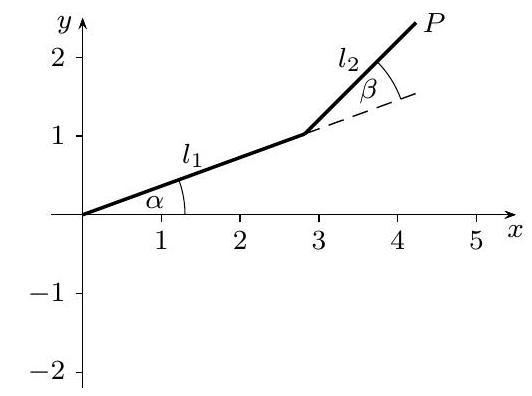
\includegraphics[max width=\textwidth, center]{2024_11_16_5119cc25e313c1f6d92ag-2}\\
ich wartości), a jeśli nie, to uzasadnij dlaczego.\\
6. Okrąg o promieniu $r$ toczy się wewnętrznie bez poślizgu po okręgu o promieniu $2 r$. Jaką linię zakreśla ustalony (dowolnie wybrany) punkt $P$ ruchomego okręgu? Wskazówka: rozważ dwa różne położenia mniejszego okręgu i sprawdź gdzie przesuwa się punkt styczności, skorzystaj ze związku między długością łuku, kątem środkowym opartym na tym łuku i promieniem okręgu.

Rozwiązania (rękopis) zadań z wybranego poziomu prosimy nadsyłać do 20.11.2022r. na adres:

\begin{verbatim}
Wydział Matematyki
Politechnika Wrocławska
Wybrzeże Wyspiańskiego 27
50-370 WROCEAW,
\end{verbatim}

lub elektronicznie, za pośrednictwem portalu \href{http://talent.pwr.edu.pl}{talent.pwr.edu.pl}\\
Na kopercie prosimy koniecznie zaznaczyć wybrany poziom! (np. poziom podstawowy lub rozszerzony). Do rozwiązań należy dołączyć zaadresowaną do siebie kopertę zwrotną z naklejonym znaczkiem, odpowiednim do formatu listu. Prace niespełniające podanych warunków nie będą poprawiane ani odsyłane.

Uwaga. Wysyłając nam rozwiązania zadań uczestnik Kursu udostępnia Politechnice Wrocławskiej swoje dane osobowe, które przetwarzamy wyłącznie w zakresie niezbędnym do jego prowadzenia (odesłanie zadań, prowadzenie statystyki). Szczegółowe informacje o przetwarzaniu przez nas danych osobowych są dostępne na stronie internetowej Kursu.

Adres internetowy Kursu: \href{http://www.im.pwr.edu.pl/kurs}{http://www.im.pwr.edu.pl/kurs}


\end{document}